\chapter{Background}
\label{background}
\epigraph{[F]or the present purposes, with the accuracy we want at first, we don't have to be very careful about defining the things very precicly.
You say \textit{``That is a terrible thing! I learnt in science you must define everything precisely.''}

\textbf{You cannot define anything precisely!} 

Otherwise you get in that paralysis of thought that comes in philosophers that sit opposite each other and one says to the other,
\textit{``You don't know what you are talking about.''} 
The other says \textit{``What do you mean by know? What do you mean by speech? What do you mean by you?''} and so on.

In order to agree to talk we just have to agree we are talking about roughly the same thing!}
{\textit{The Feynman lectures on physics, Motion, Richard Feynman, 1961.}}

%%%What is Software Evolution
Software evolution is the necessary process of changing a system to adapt the environment it exists in.
This environment is changed by the system itself, such that a feedback loop \cite{lehman1980} is created, requiring a cycle of continual evolution.
This cycle has been empirically studied and laws have been found that describe the nature of this process.  

%%%Component Evolution
To help reduce the negative effects and mitigate the risks of this evolution, Component-Based Software Engineering (CBSE) has been created. 
CBSE creates a system by composing together many encapsulated units, called software components, in a manner specified by a component model.
The component model is the specification of how software components are described and how they relate to each other to form the system.

%%%Broken into two parts
The evolution of a component based software can be broken into two different cycles; the evolution of the component, and the evolution of a component system. 
A component is evolved like a typical software system, 
but component system evolution involves changing the system at a higher granularity, by adding and removing components.
Also, a component is evolved by a developer, where a component system can be evolved by a user or stakeholder of the system.
This makes the the evolution of a component system significantly different from the evolution of an individual component.

%%%What is CDR
The act of evolving a component system can be difficult given the complex relationships between components.
These relationships create constraints on the system, that must be satisfied in order for its components to be functional.
However, given these relationships are explicitly defined the satisfaction of these constraints can be automated through a function called component dependency resolution (CDR).
This function is a powerful tool that is used to evolve a component system.

%%%Using CDR within an evolution strategy
Another difficulty in evolving a component system arises because of the different objectives that can be aimed for.
For example, a stakeholder may wish to alter very little to minimise the risk of change, or to change as much as necessary to lower the risk of being out of date.  
These objectives are taken into account and enacted in an evolution strategy, the pattern employed by the stakeholder to change and adapt their system.
This evolution strategy includes the frequency of actions to maintain or extend their systems and the criteria they take into account when evolving their system.

%%%Defining components
Component system evolution is clearly impacted by the definition used for the concept ``software component''.
The definition of a component has not been specified till this point on purpose, as it is difficult to define exactly what a component is. 
The community is still in disagreement over even fundamental aspects of software components, making it impossible to find a definition to satisfy all aspects.
However, by defining a software component with respect to component system evolution, the aspects of this evolution can be studied.
The resulting definition may conflict with others definitions of software components, 
however this method of definition allows this research to be scoped to ignore possibly superfluous arguments.

%%%Examples of component models
With respect to this definition of a component, various component models can be described.
These component models can differ by functionality, platform, or their objectives for being created.
They may also have their own CDR implementations, created to assist in their component systems evolution. 

%%%In this chapter\ldots
In this chapter; firstly the software evolution and the evolution of components and component systems is then discussed in section \ref{background.evolution}.
This section includes descriptions of component dependency resolution and the evolution strategies of stakeholders.

Then, how software components and component models are defined in this research is discussed in section \ref{background.components}.
These definitions are given with respect to component system evolution.

Finally, examples of various component models and CDR implementation are then given in section \ref{background.models}.
This includes an introduction to the Debian model, and CUDF model that are described in more detail in the following chapters.

\section{Software Evolution}
\label{background.evolution}
%%%Evolution in other contexts
Evolution is primarily used in the contexts of biology referring to the natural change of a species to survive in its environment,
and in cosmology when referring to the continual change of the universe.

%%%Software Evolution is
Software evolution is the process of change made to software system to maintain, or to extend its functionality over the systems lifetime.
This evolution is required in order to adapt to the changing environment, which is made up of stakeholders, systems, and other internal and external constraints that impact the system. 
As the system will inevitably change the environment it is in, the continual evolution in order to satisfy the stakeholders and constraints is necessary. 

%%%The nature of this evolution has been explored and laws found
The nature and fundamental laws of software evolution has be explored through empirical study of the software being evolved.
By observing the evolutionary development of many software systems and analysing the results, laws, similar to the laws of nature like gravity, can be identified.
Some of the discovered laws of this evolution are outlined by \cite{lehman1980} and \cite{lehman1997}, and presented here:

\begin{enumerate}
  \item \textit{Continuing Change:} Systems\footnote{E-type systems: software implemented in a real-world computing context} must be continually adapted else they become progressively less satisfactory
  \item \textit{Increasing Complexity:} As the system evolves its complexity increases unless work is done to reduce it
  \item \textit{Self Regulation:} the system evolves with statistically determinable trends and invariences
  \item \textit{Conservation of Organisational Stability:} The average effective activity rate to evolve a system is invariant over its lifetime
  \item \textit{Conservation of Familiarity:} As the system evolves, its incremental growth remains invariant to ensure users maintain mastery over the system.
  \item \textit{Continuing Growth:} The system must continually grow to maintain user satisfaction
  \item \textit{Declining Quality:} The quality of the system will decline unless rigorously maintained
  \item \textit{Feedback System:} As the system effects the environment it is installed in, this changes the functions it performs
\end{enumerate}

%%%These laws describe the fact that it is impossible to create a single satisfactory system, and an iterative approach is best to strive for continual satisfaction
These laws make the software engineers objective of a creating a satisfactory system impossible.
A software engineers goal is then to continually change a system to make it more satisfactory, with minimal cost and delay \cite{Lehman2006}.
This change must be accomplished while the engineer maintains intellectual control over the complexity of the system \cite{Brooks1975}, 
as the more complex a system, the greater the difficulty to change it.

This iterative process can be seen in the spiral model shown in figure \ref{spiral}, first presented by \cite{Boehm1988}.

%\usepackage{graphics} is needed for \includegraphics
\begin{figure}[htp]
\begin{center}
  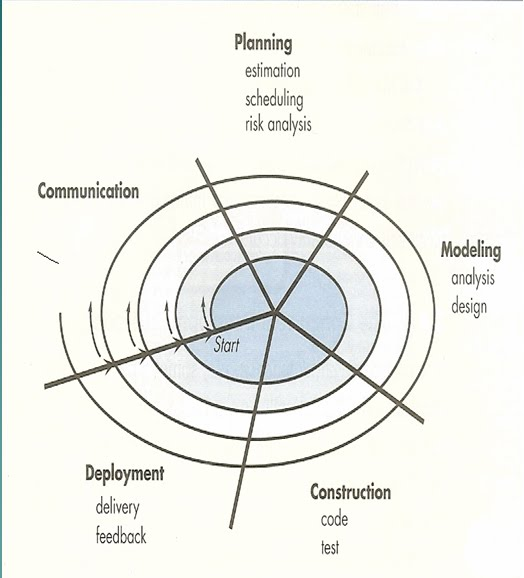
\includegraphics[width=\textwidth]{backgroundpics/spiral}
  \caption{The spiral software model}
  \label{spiral}
\end{center}
\end{figure}

%%%Figure of the iterative spiral development cycle showing its mitigation of the negative effects of the laws of software evolution
This figure shows the evolutionary cycle of software development through the stages of communication, planning, modeling, construction and deployment.
These stages are iterated ad infinitum, or until the software project reaches the end of its life. 
This is a common model used to develop a software system, and shows the necessity to consider evolution during the software development.  

%%%Therefore a software engineer, must\ldots
A software engineer must create a system that can be quickly altered to adapt to a changing environment, 
while working to reduce the inevitable complexity caused by this change.

\subsection{Component Based Software Evolution}
%%%How CBSE helps with these goals of a software developer
As stated above, the goals of a software engineer is to create a system that can be continually changed with minimal cost and delay,
while maintaining intellectual control over the systems complexity.
Towards these goals component based software engineering (CBSE) was created.

%%%What is component based software engineering
Component-based software engineering (CBSE) is considered by many to be the future for development of software systems \cite{Szyperski2002}.
It creates software systems by composing encapsulated units of execution that explicitly declare the relationships between themselves and their environment.
Many benefits are gained to the process of software evolution through using a component based system. 
The costs and time of changing a system can be reduced through more easily calculating side effects and supporting reuse within the system.
Also, using a component system reduces the complexity of the understanding and altering a system, as the system is made of higher abstracted elements. 

%%%Change in a monolithic system
Within a monolithic system any part of the system can depend on any other part without documentation or constraint.
This means that any change to the system can effect any other part in unknown and unpredictable ways.
This problem has lead to tools that analyse these dependencies to measure and mitigate their effect on the system, e.g. JDepend, Jens's tool.

%%%Change in a component system is more predicatble
Software components require the explicit definition of their relationships between one another and the system. 
With the enforcement of the encapsulation on components, this makes the effects of a change to a component based system more easily calculable.
Therefore, a components relationship to any other component in a system is calculable, making the effect of a change more easily predictable.
For instance, given a text editor component explicitly declares it's dependence on a spell checker, a change to the spell checker will have a known effect on the text editor.
Where in a monolithic system this relationship would only be implicit and the effect would then be more difficult to predict.

%%%Maximising reuse
Reuse is often cited as the main driving force of component technology, and has been empirically shown to increase the quality and productivity within software development \cite{hallsteinsen_experiences_1997}.
The amount of reuse in a system will also decrease the amount of necessary change during system evolution as there is less replicated functionality to maintain.
The greatest obstacle to reuse is the difficultly to locate and access required functionality quickly and easily \cite{ye_supporting_2001}.
As a component explicitly declares the functionality it provides and the environment it requires to function, the ability to find and use it is increased.
This can lead to greater reuse in a system and therefore less required change during evolution.
For example, if a logging component declares its provided functionality to the system, there may be no need to have another logging component installed and all components may use it.
When compared to a monolithic system, each library or class may include its own logger as their is no mechanism to reuse external functionality.

%%%Intellectual control over the complexity of the system is increased
As the systems complexity increases the ability of the engineer to make effective changes to the system decreases.
The number of units that must be looked at and the relationships between them must be considered by the engineer before a change is made.
The complexity of changing a component based system is greatly reduced due to the granularity of its construction.
The higher level abstraction of the system into components, above classes or functions, reduces the number of elements and their relationships.
At this level, the atomic evolutionary change made to a component system is the addition or removal of a component, to or from the system.

%%%Conclusion
The use of component based systems can lower the cost, time and complexity of software evolution.
Though an important distinction must now be made between the evolution of a single component, and the evolution of a component system.
This discussion is continued in the following section.

\subsection{Component Evolution vs. Component System Evolution}
%%%Evolution of a component system is made up of two cycles, the component evolution and system evolution.
Evolution is the repeated change to a software system to adapt to its environment.
There are two environments that exist when considering the evolution of a component based system; 
the environment the component exists in, and the environment that the component system exists in.
These two environments may be distinct and cause two different cycles of evolution, the evolution of individual components, and the evolution of component systems.

These separate processes, although related, have different features and aspects that must be discussed.

\subsubsection{Component Evolution}
%%%Two main differences with component evolution and typical software evolution, is the definition and testing of relationships,
%%%And the declaration and distribution of a version, not a system
The evolution of a component is similar to the evolution of a typical piece of software, using methods similar to the one present in figure \ref{spiral}.
The main exceptions is caused bt the difference that throughout evolution the explicit relationships to other components must be considered.
These relationships effect a components evolution as the related components have different evolution cycles, 
and the relationships can create a combinatorial amount of systems that component could be deployed in.

A component explicitly declares relationships to other components, therefore the development and evolution of a component will effect those that it is related to.
These effects can be passed through dependencies, and therefore must be considered throughout development.
For example, if a component $a$ is changed, and component $b$ uses $a$'s functionality, this change may effect $b$.
As the developers of $a$ do not have control over the development of $b$ the changes must be discussed, and co-ordinated to ensure that they are not detrimental to either component.

A typical piece of software is bundled together, and as a system can be tested to work before deployment.
However, as a component can be used in different contexts the specification, and testing, of the relationships is required.
As a component may contain complex relationships to many other components,
the amount of systems that the component can be deployed in can be massive.
Testing all possible systems is then impossible, which must be considered during evolution.
For example, given a text editor component depends on three versions of a spell checker, 
and four versions of a font component the total amount of possible systems is 12.
This number increases to 105 if the component system allows multiple versions of the same component to be installed.

This nature of this component evolution is explored in studies such as \cite{vasa2007patterns}, where the evolution of 5 components is empirically studied and patterns of evolution are extracted.
Other studies look at aspects like the evolution of specifications \cite{Mencl2001}, the models used to version components \cite{Stuckenholz2005},
and the general concepts related to this evolution \cite{Rhode2000}.
This area is closely related to the well studied area of software evolution, and is still an active area of research.

\subsubsection{Component System Evolution}
The evolution of a component system is accomplished through altering the structure of the component system.
This is opposed to the evolution of individual component which alters the internal structure of a single component.
This architectural level view of evolution is significantly different as it does not concern itself with the internals of the constituent components only the relationships between the components.

The core functions involved in evolving a component system are the addition and removal of components to and from the system.
These functions are executed for the same reason as the evolution of a component, for maintenance or to extend the systems functionality.
Though they differ in the fact that users, and other non-technical stakeholders can evolve the system,
there is no single metric like a version to measure the state or change to the system,
and the evolution of the system and the evolution of a component can diverge.
 
%%%Users and other non technical stakeholders can alter the system
As the evolution is more coarsely grained than that of the evolution of a single component, the necessary technological knowledge is lowered.
To evolve a single component requires programming and software development knowledge to accomplish.
However, the evolution of a piece of software from a higher level requires some knowledge of the component model and tools to change it,
though the overhead in learning this information is quite low.
For example, to maintain a component system like a Debian GNU/Linux distribution can be done through executing the command \verb+apt-get upgrade+.
To extend the system to install a component \verb+comp+ the command \verb+apt-get install comp+ can be executed.
This gives the power to evolve a system to a user.

%%%There is no version, or single metric, to describe the system state
The state a component or piece of software has evolved to can be represented by a single measurement, a version.
The state of a component system cannot be measured with a single metric as it is represented by a configuration of the versions of components that are installed in the system.
A component system then forms something like a partially ordered set, where a system can be neither more or less evolved than another.=
For instance, a system that has version 1 of component $a$ and version 2 of component $b$, is neither more or less evolved than a system with version 2 of $a$ and version 1 of $b$.
This complexity makes it difficult to compare systems, and make decisions about actions to be taken.

%%%Individual components can diverge their evolution from the system
The evolution of a component, and the evolution of a system it is in can become in conflict with each other.
As discussed above, a component is evolved disconnected from the systems it is deployed in, as a component can be used in many different contexts and systems.
When a component evolves, it may then conflict with many systems that it is part of.
For instance, a component could be developed to be used in an embedded system, but be deployed in a web-server.
The evolution of the component may continue to be evolved to adapt to the embedded environment that it is developed for,
but at some point conflicts with the web-servers requirements.
This then has the effect of stopping the evolution of that component in the web-server, or by removing that component all together.

This process of component system evolution is empirically studied in \cite{fortuna2011} by looking at the first 10 releases of the Debian Linux/GNU distribution,
and using graph metrics to analyse the evolution of the complexity of the software releases, the process can be compared to its biological counter part.
Methods to evolve component systems are discussed \cite{Ryan2005} and \cite{Luo2004},
and the mitigation of the negative effects caused by such evolution is discussed in the paper \cite{Stuckenholz2007}.
This area of research is quite new, the evolution of component systems that are occurring today are having unknown and unpredictable emergent effects that remain to be studied.

\subsection{Component Dependency Resolution}
%%%The tedious nature of satisfying component dependencies during component system evolution can be automated into a function called Component Dependency Resolution.
The relationships between component enforce the constraints on the system that must be satisfied when evolving the system.
For example, a user wants to install a new text editor component into their system, and the selected text editor has a dependency on a spell checker.
This means a spell checker component must be installed for the text editor to be functional.
As the spell checker can have its own relationships such as dependencies, 
the satisfaction of all constraints while evolving a component system can be a tedious, time consuming and error prone task.

As the components relationships are explicit, the constraints can be extracted and the process can be automated.
A function that can be used to resolve these constraints is Component Dependency Resolution (CDR) \cite{Jenson2010}.
Use of such a function lowers the cost of evolving a system, and allows for different criteria to be specified to guide evolution.
This function is implemented in many different systems, in many component models, all with the goal of automatically altering the architecture to evolve a component system.

%%%CDR lowers cost of evolution
CDR lowers the cost to evolve a system as it removes much of the effort to satisfy constraints from the user.
It also can increase the quality of the created system, as many evolutionary steps can have multiple solutions and CDR can examine and discard undesired changes.
For example, a  text editor component requires a spell checker, and three different spell checkers exist each with their own various dependencies and relationships.
To calculate a system manually may take a very long time and may not be optimal, however through the automated CDR algorithm many systems can be examined and the optimal system returned.

%%%CDR can be used at design-time and run-time on component models.
The value of this function has been seen and implemented for many different component models.
CDR can be used at design time to determine the required dependencies to build and test a project (as in Apache Maven \cite{casey_better_2008}),
at run time to evolve or extend a component-based system (as in Eclipse P2 \cite{leBerre2010}),
or it can be used to build and restructure software product lines \cite{savolainen_analyzing_2007}.
CDR is also used in package management systems, like apt-get \cite{Barth2005},
for adding, removing and updating components in package based operating systems like Ubuntu\footnote{http://www.ubuntu.com}. 

A formal definition of CDR is given in chapter \ref{cdr}, and discussion of the implementation from this study in chapter \ref{implementation}.

\subsection{Evolution Strategies}
Given any point throughout the life of a system, there are choices to be made about the systems evolution.
Should a component be removed, should one be added, should the system be upgraded and what is the way in which a system should be selected given multiple possibilities exist.
The two fears that guide these decisions are caused by the risk that change will damage the system, and the risk that not changing will leave the system out of date.

%%%The decisions that lead to an evolution strategy
The strategy that a user employs to evolve their system must take into the environment in which the system exists.
For example, if a system is a mission critical system only the necessary changes will be made to it.
Where a users desktop computer may add components for testing, and make many unnecessary changes through trial and error.
These differences are through the strategy that is used to evolve a system, the pattern to evolve the system.

%%%The risk of change to a system
When changing any software system problems can be caused by either the process of the change, or the change itself.
These problems can manifest themselves in many ways, from friction caused by an incompatibility in the system to completely destabilising the system.
They can also effect the user, as the resulting change may make the system too different from the previous system.
This problem with change is expressed in the laws of evolution stating that with each change complexity increases and quality declines.

%%%The risk of not being up to date
Why would a user ever select to evolve their system, if it is inevitable that the system will be more complex with less quality. 
The laws of evolution also state that a system must go through continually changed and grown as user satisfaction decreases with time.
As discussed, this is caused by the feedback cycle of the system effecting the environment it is made for.
For example, a system is created to digitise photos from a photo album, if it is successful the resulting change to the environment is then the large amount of digitised pictures.
The system must then adapt to service the new requirement of managing a large amount of pictures, which itself may change the environment.

How to define such a strategy and what elements must be considered is discussed in chapter \ref{strategies}.

\section{What is a Software Component?}
\label{background.components}
%%%What is a component in a larger context
A component is a natural concept that describes a part or element of a larger system or process,
a broad definition of a component is ``components ca be composed together''.
They are usually physical, as in electrical or mechanical components, where their properties and how they are composed are documented to be used in construction.
Typically, components can be used in many different contexts, e.g. an resistor component, they can be used in electrical systems from space stations to cellphones.   

%%%Some history to software components mentioning McIlroy's 1969 paper \cite{McIlroy1969}
Software components ideals can be traced to \cite{McIlroy1969}, where the author describes his ideas industrializing software engineering through a software component sub-industry. 
These components are made through the decomposition of software into discreet units with explicitly stated interfaces and behaviours.
However, there is still much debate over how to define what a software component is, and what features it should have.

%%%Discussion of articles where Szyperski and Meyers discuss give their versions of what a component is.
A discussion between two leading researchers in component software, Bertrand Meyer and Clemens Szyperski, highlight this difficultly of defining exactly what a software component is. 
They describe across multiple articles \cite{Meyer1999,Szyperski2000a, Szyperski2000, Meyer2000,} the definitions of what a software component is and the importance of their use.

%%%Szyperski's definition
Szyperski defines components in \cite{Szyperski2002} as having three characteristic properties:
\begin{enumerate}
  \item a unit of independent deployment
  \item a unit of third party composition
  \item has no externally observable state
\end{enumerate}

%%%Meyers Definition
Meyer's definition of software components is enumerated as:
\begin{enumerate}
  \item May be used by other software elements (clients)
  \item May be used by clients without the intervention of the components
  developers
  \item Includes a specification of all dependencies (hardware and software
  platform, versions, other components)
  \item Includes a precision specification of the functionality it offers
  \item Is usable on the sole basis of that specification
  \item Is composable with other components
  \item Can be integrated into a system quickly and smoothly
\end{enumerate}

%%%Using a component model
Others, like Heineman and Councill \cite{heineman2001component} have stated that components must conform to a component model, 
\begin{quotation}
A software component is a software element that conforms to a component model and can be independently deployed and composed without modification according to a composition standard.
\end{quotation}

Defining a component model as:
\begin{quotation}
A component model defines a set of standards for component implementation, naming, interoperability, customization, composition, evolution, and deployment.
\end{quotation}

%%%Other differences, architectural/implementation
Exactly what is, and what is not a software component is then in dispute amongst the community.
A definitive description of a software component is elusive \cite{vasa2007patterns}.
As such, many different components models have been developed, each targeting various domains with different functionality and technical aspects.
This diversity has inspired a classification approach from \cite{Crnkovic2011}, where components and component models are classified into a scheme.
This effort highlights the difficulty in creating an exact definition of a software component. 

%%%It is difficult to define a natural concept such as component with a set of fixed enumerable features.
These problems with exactly defining a software component may stem from the fact that ``component'' is a natural concept.
The problem, observed from the area of formal concept analysis \cite{Ganter1999} by \cite{Szyperski2002}, is that it is impossible to

\begin{quotation} 
``enumerate a fixed agreeable set of features that is necessary and sufficient for a natural concept such as component.'' 
\end{quotation}

%%%Our egotistical view of components is defined with relation to Component Dependency Resolution.
However, a definition can be found, not by feature enumeration but through stating the intention for the concept and exploring the technically inevitable consequences \cite{Szyperski2002}. 
As the intention of this study is to investigate component dependency resolution and evolution strategies,
the definition of software component used will be in respect to these aspects.

%%%This will not fit all views of what a component is (no definition will), but it eliminates unnecessary arguments so we can focus on CDR
This view of a software components definition will not agree with every persons view of what a software component is, but (as described above) no view can.
By only looking at aspects that are necessary for our topic, the arguments over unnecessary semantics are eliminated, leaving only the core aspects of this research. 

\subsection{Software Component}
The definition of a software component is given with respect to the evolution of the system using component dependency resolution.
Both these areas will be explored further in this chapter, however it is most important to first define the concept of ``software component''.
This definition specifies requirements on the component model that ensure it is applicable in this research.

For CDR to be used with a component system, there are two core requirements, the component model must:
\begin{enumerate}
  \item require the explicit definition of dependencies between components
  \item include mechanisms in which to programmatically compose or evolve a component system
\end{enumerate}
This definition leaves undefined many aspects of component model, however these are ignored as they are not related to CDR of component system evolution.

%%%A component must have explict (computer readable) requirements on the context in which it can be used. Different from COTS requirements which are meant to be human readable.
To automate the resolution of dependencies between components, these dependencies must be explicitly defined and computer readable.
These dependencies constraint the environment in which the component can be executed.
As CDR requires the ability to calculate systems that will function, this requirement is necessary.

%%%The component model should specifiy mechanisms to support evolution of the system; e.g. the addition and removal of components from a composition.
The creation or evolution of a component system must be able to be automated for CDR to be usable.
This means that CDR should have the ability to add, remove and replace components in a system, and create a functioning system.
These actions can occur at either at compile-time or run-time of the system.
As CDR would evolve a system automatically, these actions must be able to be enacted either through a function call, or well defined command interface.

%%%Aspects such as semantics of composition, distribution, development, are outside the scope of CDR, therefore ignored in this definition (that is not to say they are unimportant).
The classification, from \cite{Crnkovic2011}, of a component model is partially described as:
\begin{itemize}
  \item Lifecycle 
  		\begin{itemize}
	  		\item Modelling
	  		\item Implementation
	  		\item Packaging
	  		\item Deployment
		\end{itemize}
	\item Construction
		\begin{itemize}
	  		\item Interface Specification
	  		\item Binding
	  		\item Interactions 
		\end{itemize}
	\item Extra Functional Specifications
		\begin{itemize}
	  		\item Management
	  		\item Specification
	  		\item Composability
		\end{itemize}	
\end{itemize}  
This list displays the complexity in defining a component model.
In this classification scheme, the two aspects that are included in this definition are lifecycle deployment for the evolution of a component system, 
and construction interface specification for the explicitly defined dependencies.
All the other aspects that practically must be defined, are here ignored as their definition is superfluous to the core topic of this research.

These core aspects will be explored in the following sections, with examples of different component models and CDR implementations being presented.


\section{Component Models}
\label{background.models}
%%%Some core component models are described, and their dependencies and evolution are discussed
Given the definition of a software component for this research, some current component models are described and discussed.
These models come from industry (OSGi, Eclipse Plugins, Fractal, Maven), open source community (Debian, RPM) and academia (SOFA2).

The typical mechanism in which components, from these frameworks, describe their relationships is through meta-data files.
These files contain what the component requires and provides, as well as other information like versions and provider details.
The way in which these component models express their relationships will be described.

Typically, the component model also provides a mechanism to alter the system of components.
This is usually a low level interface, such that the addition of a component is an atomic step and does not lead to the addition of other components.
These basic mechanisms are usually abstracted to be more usable, by automatically resolving dependencies using a CDR implementation.
These implementations have their various criteria and strategies to evolve their component systems.
When applicable the mechanisms, CDR implementations and their criteria will be discussed.

Together, the declaration of the component relationships, and the mechanisms to alter the system mean these models fall within our component definition.

To compare these component models, the relationship of a text editor component, that requires a spell checker component is used.
This is a simple example, however it highlights the possible differences in these models.


\subsection{OSGi}
%%%What OSGi is? Bundle Service
OSGi is a mature component model from the OSGi Alliance.
It has a significant presence in industry \cite{Kriens2008} from organizations like the Eclipse Foundation with their Equinox framework and Apache with Felix framework.

OSGi components are refereed to as bundles, these contain JVM classes with meta-data describing their relationships.
A notable difference between OSGi and other component frameworks is that it separates the unit of deployment, the bundle, and the unit of deployment the service.
These services exist on a separate layer to the bundles, each service is created at run-time and is represented by a Java object.
This service layer allows third-party frameworks to describe service relationships, e.g. Spring Dynamic Modules.
These relationships and the interaction with services make themselves a component, under our definition.
A standard way of interacting with this layer is defined in the OSGi compendium is Declarative Services (DS).

OSGi is implemented to allow dynamic interaction, the addition and removal of bundles at run-time.
This can be done through a console implemented in the Equinox OSGi framework, this enables user interaction.

An example of a bundle which defines a text editor that depends on a spell checker is described in figure \ref{osgibundle}.

\begin{figure}[htp]
\begin{center}
\begin{alltt}
Bundle-Name: TextEditor
Bundle-Vendor: Graham Jenson
Bundle-SymbolicName: nz.geek.maori.textEditor
Bundle-Version: 0.0.1.alpha
Bundle-RequiredExecutionEnvironment: J2SE-1.4
Export-Package: nz.geek.maori.textEditor;version="0.0.1.alpha"
Require-Bundle: nz.geek.maori.fonts
Import-Package: nz.geek.maori.spellchecker;version>"0.0.1"
\end{alltt}
  \caption[OSGi Meta-data]{Example of OSGi Meta-data}
  \label{osgibundle}
\end{center}
\end{figure}

%%%OSGI Meta data description
This meta-data shows the name, version and vendor of the component, as well as the exported packages (referring to Java packages) which are able to be used by other components.
The \verb+Require-Bundle+ key expressed the direct dependence on another bundle.
The \verb+Import-Package:+ key expresses the dependence on a package provided by a bundle and not on the bundle itself.

This meta-data only contains the necessary relationships to install a bundle, not what it requires to be functional.
This information is in the service layer, described by the meta-data available in DS.
An example of this meta-data is in figure \ref{dsmetadata}.

\begin{figure}[htp]
\begin{center}
\begin{alltt}
<?xml version="1.0"?>
<component name="textEditor">
    <implementation class="nz.geek.maori.textEditor.TextEditorImpl"/>
    <service>
        <provide interface="nz.geek.maori.textEditor.TextEditor"/>
    </service>
    <reference name="spellChecker"
        interface="nz.geek.maori.spellchecker.SpellChecker"
        bind="setSpellChecker"
        unbind="unsetSpellChecker"
        cardinality="0..1"
        policy="dynamic"/>
</component>
\end{alltt}
  \caption[OSGi Declarative Services]{Example of OSGi Declarative Services meta-data}
  \label{dsmetadata}
\end{center}
\end{figure}

This meta-data includes references to implementation elements like interfaces that are provided and required, and methods to interact with the services.
These relationships can have cardinalities, e.g. a text editor can use multiple spell checkers, and other programmatic features.
The goal of this service meta-data, like the bundle meta-data, is to express the environment in which this component can be used by others.
The \verb+service+ tag describes the services provided, and the \verb+reference+ tag expresses a dependence on another services.

%%%DS provides no versioning
One aspect of DS that is lacking, is the ability to explicitly version services.
The version of the bundle that is providing the service and the version of the package that is provided by the bundle, implicitly version the service being provided.
However, for the evolution of a component model, some type of versioning is required to give a relative timestamp of it's development.
This may make the evolution of these services difficult to predict, and therefore difficult to use CDR to evolve them. 


\subsubsection{Evolution of OSGi}
The programmatic evolution of an OSGi system is defined in the interfaces created by the OSGi alliance \footnote{http://www.osgi.org/javadoc/r4v43/}, therefore are OSGi framework agnostic.
The installation and removal of both the bundles and services from the OSGi system are defined as such:
 
\begin{itemize}
  \item To install a bundle: \verb+org.osgi.framework.BundleContext.install+
  \item To uninstall a bundle: \verb+org.osgi.framework.Bundle.uninstall+
  \item To register a service: \verb+org.osgi.framework.BundleContext.registerService+
  \item To unregister a service: \verb+org.osgi.framework.ServiceRegistration.unregister+
\end{itemize}

OSGi therefore has the necessary elements in order to be considered a component model for this research. 
It has the ability to explicitly describe relationships between either bundles or services, and to install and remove bundles from the system.

\subsubsection{OSGi Bundle Repostiory}
%%%The OBR proposed by Peter Kriens and Richard Hall, is a meta data format for OSGi bundle resolution
A CDR implementation for OSGi was proposed by Peter Kriens and Richard S. Hall in RFC-0112 \cite{the_osgi_alliance_rfc-0112_2006}.
This is called the OSGi Bundle Repository and consists of collection of components documented in an XML format and documentation which describe a component as a resource.
An example of this document is shown in figure \ref{obrmetadata}.

\begin{figure}[htp]
\begin{center}
\begin{alltt}
<repository name='OBR REP' time='123'> 
  <resource version='0.0.1' name='nz.geek.maori.textEditor' 
  uri='nz.geek.maori.textEditor.0.0.1.jar'> 
    <require optional='false'  multiple='false'  name='package' 
        filter='(&amp;(package=nz.geek.maori.spellChecker)(version&gt;=1.0.0))'> 
      Import package nz.geek.maori.spellChecker ;version=1.0.0 
    </require> 
  </resource> 

  <resource version='1.0.0' name='nz.geek.maori.spellChecker' 
  uri='nz.geek.maori.spellChecker-1.0.0.jar'> 
    <capability name='package'> 
      <p v='nz.geek.maori.spellChecker' n='package'/> 
      <p v='1.0.0' t='version' n='version'/> 
    </capability> 
  </resource> 

</repository>
\end{alltt}
  \caption[OSGi Bundle Repository markup example]{Example of OSGi Bundle Repository meta-data}
  \label{obrmetadata}
\end{center}
\end{figure}

This meta-data was designed so that it can merge such meta-data as described in figures \ref{osgibundle} and \ref{dsmetadata}.
This then would be a complete model at both the OSGi bundle and service layers, to be used by CDR to create a complete system. 

OBR has been seen as a solution to to simplify deployment of OSGi applications \cite{jung_integrating_2007}, 
distribution and deployment to embedded ubiquitous systems \cite{jung_embedded_2006}, 
smart home applications \cite{gouin-vallerand_managing_2007} and 
dynamic distribution of drivers \cite{kriens_osgi_2008}. 

The most mature implementation of OBR client is offered by Apache, it is bundled with their core OSGi framework, Apache Felix. 
This can be used with any of the large public or private OBR collections of bundles.
An example of one such public repository is the Paremus repository\footnote{http://www.osgi.org/Repository/} which contains (as of December 2011) over 2000 bundles.

The specification of OBR does not define the criteria by which evolutions are made to the system.
The strategy used is then described outside of the specification in the Apache OBR\footnote{http://felix.apache.org/site/apache-felix-osgi-bundle-repository.html accessed 6/12/2011} help page,

\begin{quotation}
\[OBR\] might have to install new bundles during an update to satisfy either new dependencies or updated dependencies that can no longer be satisfied by existing local bundles. 
In response to this type of scenario, the OBR deployment algorithm tries to favor updating existing bundles, if possible, as opposed to installing new bundles to satisfy dependencies.
\end{quotation}

This shows that when updating a system of bundles, newer bundles may be installed although currently installed bundles are preferred.

\subsection{Eclipse Plugins}
%%%What is Eclipse
Eclipse is a widely used IDE and an extencible plugin platform for createing Java applications.
It is built on top of the OSGi framework, but ignore OSGi's service layer and re-implements it with its own Eclipse plugin runtime.
Therefore, like the declaritive services, the distruted elements are OSGi bundles but the run time elements are plugins.

These plugins are defined using extensions and extension points, these are the relationships between the plugins.
An example of the meta-data describing a plugin is given in figure \ref{eclipseplugin}. 

\begin{figure}[htp]
\begin{center}
\begin{alltt}
<?xml version="1.0"?>
<plugin
    name="Text Editor"
    id="nz.geek.maori.textEditor"
    version="0.0.1.alpha"
    provider-name="Graham Jenson">
    
    <requires>
        <import plugin="nz.geek.maori.fonts"/>
    </requires>

    <runtime>
        <library name="texteditor.jar"/>
    </runtime>
    
    <extension-point id="nz.geek.maori.spellchecker" 
        name="Spell Checker" 
        schema="spellchecker.exsd"/>
</plugin>
\end{alltt}
  \caption[Eclipse Plugin meta-data]{Example of an Eclipse Plugin plugin.xml meta-data file}
  \label{eclipseplugin}
\end{center}
\end{figure}

This plugin defines the name, version and provider of the plugin, and using the tags \verb+requires+ defines the requirements of this plugin to function.
The \verb+extension-point+ tag defines not only what the plugin provides, but also the required information it requires in order to provide it, described in a schema.
This is a special feature of the Eclipse plugin framework, as other component models generally do not specify these parameters on this type of relationship. 

The schema of an extension point, as shown in figure \ref{eclipseextensionschema}, describes the elements to use an extension.

\begin{figure}[htp]
\begin{center}
\begin{alltt}
<schema targetNamespace="null" xmlns="http://www.w3.org/2001/XMLSchema">
 <element name="spellchecker">
  <complexType>
   <attribute name="spellchecker" type="string" use="required">
    <annotation>
     <appinfo>
      <meta.attribute kind="java" basedOn=":nz.geek.maori.ISpellChecker"/>
     </appinfo>
    </annotation>
   </attribute>
  </complexType>
 </element>
</schema>
\end{alltt}
  \caption[Eclipse Plugin extension point schema]{Example of an Eclipse Plugin extension point schema file}
  \label{eclipseextensionschema}
\end{center}
\end{figure}

In this description, this extension point requires a string that describes a java class that implements \verb+nz.geek.maori.ISpellChecker+.
This is the only requirement for this extension point, but other parameters of types, e.g. Boolean, integer, can be defined.

\subsubsection{Eclipse Evolution}
The programmatic evolution of an Eclipse system is through the use of the previously OSGi methods and with interaction with the plugin registry.

As an eclipse plugin is an OSGi bundle, and the eclipse framework uses OSGi, the methods for installing and removing a plugin are the same as for OSGi.

The extensions and extension points, for an Eclipse system, can be altered in the plugin registry.
This is the storage of all the extensions and extension points for interaction, and the core interaction with this layer of the plugins.
The methods used to add and remove these are then:

\begin{itemize}
  \item add extensions and extension points described in an XML file : \verb+org.eclipse.core.runtime.IExtensionRegistry.addContribution+
  \item remove extension: \verb+org.eclipse.core.runtime.IExtensionRegistry.removeExtension+
  \item remove extension point: \verb+org.eclipse.core.runtime.IExtensionRegistry.removeExtensionPoint+
\end{itemize}

The Eclipse plugin system can therefore be defined as a component system in this study.
It contains the necessary explicit relationships, and the programmatic evolution requirements necessary for CDR to be used.

\subsubsection{Eclipse P2}
%%%The Eclipse P2 Solver, by Le Berre and Rapicault
Eclipse P2 \cite{le_berre_dependency_2009}, \cite{leBerre2010} is the provisioning system for the Eclipse IDE platform.
It provides the interaction to alter an Eclipse based component system. 
It is implemented using a Boolean Satisfiability solver, called SAT4J.
This method of implementation has become a typical way of implementing CDR, explored in \cite{Berre2008}, and further discussed in chapter \ref{implementation}.

Eclipse P2 is mainly accessed through the Eclipse user interface, where the user can select to update the entire system, or install a component.

Some of the criteria used by Eclipse P2 to evolve the system are described in \cite{le_berre_dependency_2009} and \cite{leBerre2010}:
\begin{enumerate}
  \item minimise the amount of components installed that have no dependency to them 
  \item minimise the removal of already installed components
  \item minimise the age of the installed components
  \item minimise changing an installed component if they are unrelated to the request being made
\end{enumerate} 

Some of the Eclipse specific criteria have been removed from this list.
The presented criteria are general enough to be selected for any component system, and can be reused.


\subsection{Fractal}
Fractal is a component model developed by France Telecom R\&D and INRA.
It is a specification that is designed to be programming language independent, unlike OSGi or Eclipse.
The most notable aspect, and the reason for its name, is that a components can be composed together to make a new component.
This recursive nature of composition, actually means the the system of components is itself a component.

An example of meta-data to define a Fractal component is given in figure \ref{fractalmetadata}.

\begin{figure}[htp]
\begin{center}
\begin{alltt}
<?xml version="1.0" encoding="ISO-8859-1" ?>
<!DOCTYPE definition PUBLIC 
    "-//objectweb.org//DTD Fractal ADL 2.0//EN" 
    "classpath://org/objectweb/fractal/adl/xml/basic.dtd">

<definition name="textEditorComponent">
  <interface name="textEditor" role="server" signature="nz.geek.maori.textEditor"/>
  <interface name="spellChecker" role="client" signature="nz.geek.maori.spellChecker"/>
  <content class="nz.geek.maori.textEditorImpl"/>
</definition>
\end{alltt}
  \caption[Fractal ADL Example]{Example of a simple Fractal ADL file}
  \label{fractalmetadata}
\end{center}
\end{figure}

This meta-data describes the relationship between components as the metaphor of client and server.
The interface tag with the role attribute assigned to ``server'', defines the provided functionality of the component.
The interface tag with the role attribute assigned to ``client'' then defines the required functionality of the component.  

An example of the definition of a recursive component can be seen in figure \ref{fractalrecursve}.

\begin{figure}[htp]
\begin{center}
\begin{alltt}
<?xml version="1.0" encoding="ISO-8859-1" ?>
<!DOCTYPE definition PUBLIC 
    "-//objectweb.org//DTD Fractal ADL 2.0//EN" 
    "classpath://org/objectweb/fractal/adl/xml/basic.dtd">

<definition name="textEditorWithSpellCheckerComponent">
  <interface name="textEditorWithSpellChecker" role="server" signature="nz.geek.maori.textEditorWSC"/>
  <component name="textEditorComponent">
    <interface name="textEditor" role="server" signature="nz.geek.maori.textEditor"/>
    <interface name="spellChecker" role="client" signature="nz.geek.maori.spellChecker"/>
    <content class="nz.geek.maori.textEditorImpl"/>
  </component>
  <component name="spellCheckerComponent">
    <interface name="spellChecker" role="server" signature="nz.geek.maori.spellChecker"/>
    <content class="nz.geek.maori.spellChecker.SpellChecker"/>
  </component>
  <binding client="this.textEditorWithSpellChecker" server="textEditorComponent.textEditor"/>
  <binding client="textEditorComponent.spellChecker" server="spellCheckerComponent.spellChecker"/>
</definition>
\end{alltt}
  \caption[Fractal ADL Example]{Example of a simple Fractal ADL file}
  \label{fractalmetadata}
\end{center}
\end{figure}

In this description of a recursive component structure, as well as defining both the text editor and spell checker components it also defines and instructs their relationships.
The tag \verb+definition+ is then used as a container of components, rather than the deifnition of a single component.
This composite component defines that it provides a service of \verb+textEditorWithSpellChecker+.
To provide this the spell checker must be bound (described in the tag \verb+binding+) to the text editor,
and the text editors provided interface bound to the output interface. 

The programmatic evolution of a Fractal component system can differ between implementations.
To simplify this, only the Java implementation is described. 

\subsubsection{Fractal Evolution}
In this implementation the methods to edit the configuration are\footnote{http://fractal.ow2.org/current/doc/javadoc/fractal/}:
\begin{itemize}
  \item to create a component: \verb+org.objectweb.fractal.api.factory.GenericFactory.newFcInstance+
  \item to add a component to a composite: \verb+org.objectweb.fractal.api.control.ContentController.addFcSubComponent+
  \item to remove a component from a composite: \verb+org.objectweb.fractal.api.control.ContentController.removeFcSubComponent+
\end{itemize}

There are two points that may make the evolution of Fractal component model particularly difficult,
the recursive nature of Fractal, and the lack of required version information about components and composites.

%%%Fractal requires not only the selection of components but the configuration
Given the recursive nature of the components described, any system may provide the same functionality with the same components in a combinatorial number of configurations.
Therefore, not only would a CDR algorithm require to select a set of components but also provide or select the composites to configure them.
The simplest solution to this problem is to ignore the recursive nature of this component model,
and use a CDR algorithm to create exactly one composite with all components in it.
More difficult solutions could be created by reusing user composites, or analyzing the graph structure and grouping into clusters using algorithms like the one presented in \cite{dietrich2008cluster}.

Another aspect of Fractal that will make the automatic evolution of systems difficult will be the lack of versioning information.
Like DS, this component model doesn't not explicitly require the version of the component and the interfacs they provide.
As versions are typically the atomic unit of evolution, the process of selecting a newer version will be made more difficult if not impossible. 

\subsection{Maven}
Maven is a build automation tool, designed to be programming language agnostic but primarily used with Java.
The core component aspect of Maven is that it can dynamically select and download files from a repository to be used to build a system.
Although Maven is built using a plugin architecture, the focus in this section is on the use of Maven as a component model and not Maven itself.

A system is defined using a Project Object Model (POM) file, an example given in \ref{mavenmetadata}. 

\begin{figure}[htp]
\begin{center}
\begin{alltt}
<project xmlns="http://maven.apache.org/POM/4.0.0"
  xmlns:xsi="http://www.w3.org/2001/XMLSchema-instance"
  xsi:schemaLocation="http://maven.apache.org/POM/4.0.0
                      http://maven.apache.org/xsd/maven-4.0.0.xsd">

  <groupId>nz.geek.maori</groupId>
  <artifactId>textEditor</artifactId>
  <version>0.0.0.alpha</version>

  <dependencies>
    <dependency>
      <groupId>nz.geek.maori</groupId>
      <artifactId>spellChecker</artifactId>
      <version>[0.0.1,1.0.0)</version>
      <type>jar</type>
     </dependency>
  </dependencies>
</project>
\end{alltt}
  \caption[Maven POM file]{Example of a Maven POM file}
  \label{mavenmetadata}
\end{center}
\end{figure}

This model defines the components namespace using the \verb+groupId+ tag, the name using the tag \verb+artifactId+, and the version.
It also defines the dependencies on other projects through the \verb+dependency+ tag,
where it states that it depends on the artifact \verb+spellChecker+ from versions 0.0.1 to (but excluding) version 1.0.0.

\subsubsection{Maven Evolution}
The use of Maven as a development time component model, does not exclude it from the definition of being a component model in this study.
Though it puts it in a unique situation, where it does not evolve a component system by altering it, but by recompiling and replacing it.
Therefore, the evolution of a Maven based system is done simply by selecting the projects to build, and using Maven to compile them into a system. 

Another core difference from the other presented component models is that Maven POM objects do not declare what they provide.
For example, an OSGi bundle can declare provided packages and a Fractal component declares provided interfaces, where a Maven project can only provide itself.
This will simplify a CDR algorithm by not having to resolve another layer of dependencies.

\subsection{Debian Packages}
Debian is a GNU/Linux based operating system provided by the Debain Project \citep{Barth2005}.
This operating system most prominent feature is that it is composed of packages, unit of deployment with explicit dependencies.

Each package is defined using a control file, an example presented in figures \ref{debianmetadatate} and \ref{debianmetadatasc}.

\begin{figure}[htp]
\begin{center}
\begin{alltt}
Package: textEditorPackage
Version: 0.0.1.alpha
Depends: spellChecker
Conflicts: otherTextEditorPackage
\end{alltt}
  \caption[Debian Control file for Text Editor]{Example of a Debian Control File for Text Editor}
  \label{debianmetadatate}
\end{center}
\end{figure}

\begin{figure}[htp]
\begin{center}
\begin{alltt}
Package: spellCheckerPackage
Version: 1.0.0
Provides: spellChecker
\end{alltt}
  \caption[Debian Control files for Spell Checker]{Example of a Debian Control File for Spell Checker}
  \label{debianmetadatasc}
\end{center}
\end{figure}

These control files describe two packages, a text editor and spellChecker, they are organised into key/value pairs seperated by the ``:'' character.
The text editor states using the \verb+Depends+ key that is requires a spellChecker to be installed, 
and through the \verb+Conflicts+ key states that it cannot be installed with another text editor.
The spell checker package defines that it provides a spell checker  using the \verb+Provides+ key.

The semantics of these control files is further described in the section \ref{DebToCUDF}.

One aspect that differentiates the Debian package model from the many other models, is that it does not specify the rules of composition between components.
That is, there is no formal specification of the semantics of the communication and relationships between packages.
For instance, OSGi bundles exist in a very constrained environment that manages their interactions, dependning on another bundle gives has run-time implications.
For Debian, the dependence has no run-time effects, only whether the package is functional or not.
The way in which a package, uses or communcates with a depended upon package is then defined between the packages and not in the component model.

Since the composition of packages is not an aspect of this study, this is a valid component model, though some may disagree.


\subsubsection{Debian Evolution}
The application dpkg is the command line tool use to modify a Debian package system.

The commands to modify a Debain package system are:
\begin{itemize}
  \item to add a package: dpkg --install <package file>
  \item to remove a package: dpkg --remove <package>
\end{itemize}

These commands define the atomic actions to change a Debain system.
They can be executed from other applications through the command line, this makes them programming language independent and easily accessible. 

\subsubsection{Apt-get}
The application dpkg can only remove and add a single component at a time, it does not resolve the dependencies of the component.
There are many applications that can resolve these dependencies on a Debian system, the default and most popular solution is through the apt pacakage.
This package is built on top of dpkg, to provide an interface to simplyfy and extend its functionality.

From the Apt manual:
\begin{quotation}
\begin{alltt}
apt-get is the command-line tool for handling packages, and may be
       considered the user's "back-end" to other tools using the APT library.
       Several "front-end" interfaces exist, such as dselect(1), aptitude(8),
       synaptic(8) and wajig(1).
 \end{alltt}
\end{quotation}

Apt is purely a command line tool, which provides the necessary tools to efficiently allow the user to evolve their system.

The criteria it uses to update the system and install components into the system is explained in the apt-get manaual:

\begin{quotation}
\begin{alltt}
       under no circumstances are currently installed packages removed, or packages
       not already installed retrieved and installed. New versions of
       currently installed packages that cannot be upgraded without
       changing the install status of another package will be left at
       their current version.
 \end{alltt}
\end{quotation}

Another application that extends APT further is Aptitude \cite{Burrows2005}.
This application adds a basic user interface to APT and also increases functionality in aspects like locating and removing redundant packages. 

%%%TODO Write about the crtieria that are used to insall and update components

\subsection{SOFA 2.0}
Software Appliance (SOFA) is a component model developed at Charles University in Prague.
A component in the SOFA framework is defined by it's frame, which contains the meta-data of what the component requires and provides.
Like Fractal, SOFA is a recursive component model, allowing for a composite of components to be treated as a single component.

An example definition of a frame is given in figure \ref{SOFAmetadata}.

\begin{figure}[htp] 
\begin{center}
\begin{alltt}
<?xml version="1.0"?>
<frame name="nz.geek.maori.textEditor">
  <requires name="spellChecker" itf-type="sofatype://nz.geek.maori.spellChecker"/>
</frame>

<?xml version="1.0"?>
<frame name="nz.geek.maori.spellChecker">
  <provides name="spellChecker" itf-type="sofatype://nz.geek.maori.spellChecker"/>
</frame>
\end{alltt}
  \caption[SOFA ADL files]{Example of a SOFA ADL Files}
  \label{SOFAmetadata}
\end{center}
\end{figure}

This meta-data descirbes two components, a text editor and a spell checker, using the tag \verb+frame+.
The sub elements \verb+requires+ and \verb+provides+ describes their relationship through an externally defined interface with the namespace \verb+sofatype://nz.geek.maori.spellChecker+.
This interface is defined using an Architecture Definition Language (ADL) and added to a repository to be re-used. 


\subsubsection{SOFA Evolution}
SOFA 2.0 is an extension of the SOFA framework, with new services including dynamic reconfiguration for dynamic evolution of an architecture at runtime. 
Unlike other component systems,
it only allows for controlled evolution; 
Many component models allow the change of the component system on a fine grained level of adding or removing a component.
However this model only allows more grainular changes to be made to the system, these changes must conform to specified evolution patterns.
This restriction is meant to increase the manageability and predictability of a component systems evolution. 

Three evolution patterns are predefined: factory pattern, removal pattern, and service access pattern.
As its name suggests, in factory pattern a designated component serves as a component factory. 
The removal pattern serves for destroying of a component previously dynamically created.
The service access pattern allows for the access to external services.
These patterns are further discussed in \cite{Hnetynka2006}.


\subsection{Common Upgradeability Description Format}
%%%CUDF model created for compeition
Many component models share similar properties:
\begin{itemize}
  \item a component name
  \item a component version
  \item description of what the component provides
  \item description of what the component requires
\end{itemize} 

By creating an abstraction of these models, that only contains the information that is necessary for CDR, different CDR implementations can be compared.

The Common Upgradeability Description Format (CUDF) model is defined as an abstract representation of the problem found when evolving a package based system, e.g. Debian.
It was created by the Mancoosi project to foster interest and competition in creating solvers for upgrading problems faced by Free and Open Source Software (FOSS).
This specification contains the necessary detail to express the core aspects of evolution, and an extensible syntax to allow for component model specific detail. 
CUDF allows the description of many CDR problems in a single format, and the use of various CDR implementations to solve them. 

%%%No concrete components, but fits our definition
There is no concrete component representation, as it was not designed to be an executable component model.
This means that there is no detail of how to execute the component system, or other implementation focused details that are necessary for the other presented component models.

In figure \ref{CUDFmetadata}, an example of a CUDF problem is presented.

\begin{figure}[htp] 
\begin{center}
\begin{alltt}
package: textEditor
version: 1
depends: spellCheckerService

package: spellChecker
version: 2
provides: spellCheckerService

request:
install:textEditor

\end{alltt}
  \caption[CUDF meta-data file]{Example of a CUDF problem file}
  \label{CUDFmetadata}
\end{center}
\end{figure}

The CUDF file is defined using key/value pairs, where each component is defined using the two tags \verb+package+ and \verb+version+.
This file does not only represent the components but also the evolutionary change with the tag \verb+request+.
Further definition of the syntax and semantics of CUDF is in chapter \ref{cdr}, as it is used extensively throughout this study.

\subsubsection{Mancoosi MPM}
%%%The mancoosi Modular Package Manager uses CUDF, currently going through the process in the Debian component repository
The CUDF component model is defined especially to compare CDR implementations, therefore many various implementations exist.
Some of these will be discussed in the latter chapter \ref{implementation}.
However, here only the default implementation , Modular Package Manager \citep{abate2011} (MPM), is discussed.
This implementation was created by the Mancoosi organisation to explore the possibility of using CUDF to evolve real systems.

In the study from \cite{abate2011}, this package manager was compared against other component solvers, such as apt and aptitude, and shown to be an improvement.
This CDR implementation is the first to allow the user to completely specifiy the criteria by which the solver selects a system.
In the study the solver first minimised the amount of packages removed from the system, and then minimised the amount of packages changed in the system.
Further discussion of these criteria and how they are combined is discussed in chapter \ref{strategies}. 

\section{Summary}

In this chapter, first the evolution of software was discussed, and the nature and laws of this process described.
The area of component based software engineering and the benefits its provides to the process of software evolution.
The evolution of a component based system, through the individual component evolution and the evolution of a component system is discussed
and how component dependency resolution and evolution strategies are used to evolve a component system.
Given these goals of this study, software components are defined, and examples given that fit this deinfition.

In the next chapter the evolution of a component system is further defined.













